Die gewählten \textit{Cluster} nach den Kriterien aus Abschnitt \ref{s3s1s2} bestehen fast ausschließlich aus Photonen.
\begin{figure}[t!]
\centering
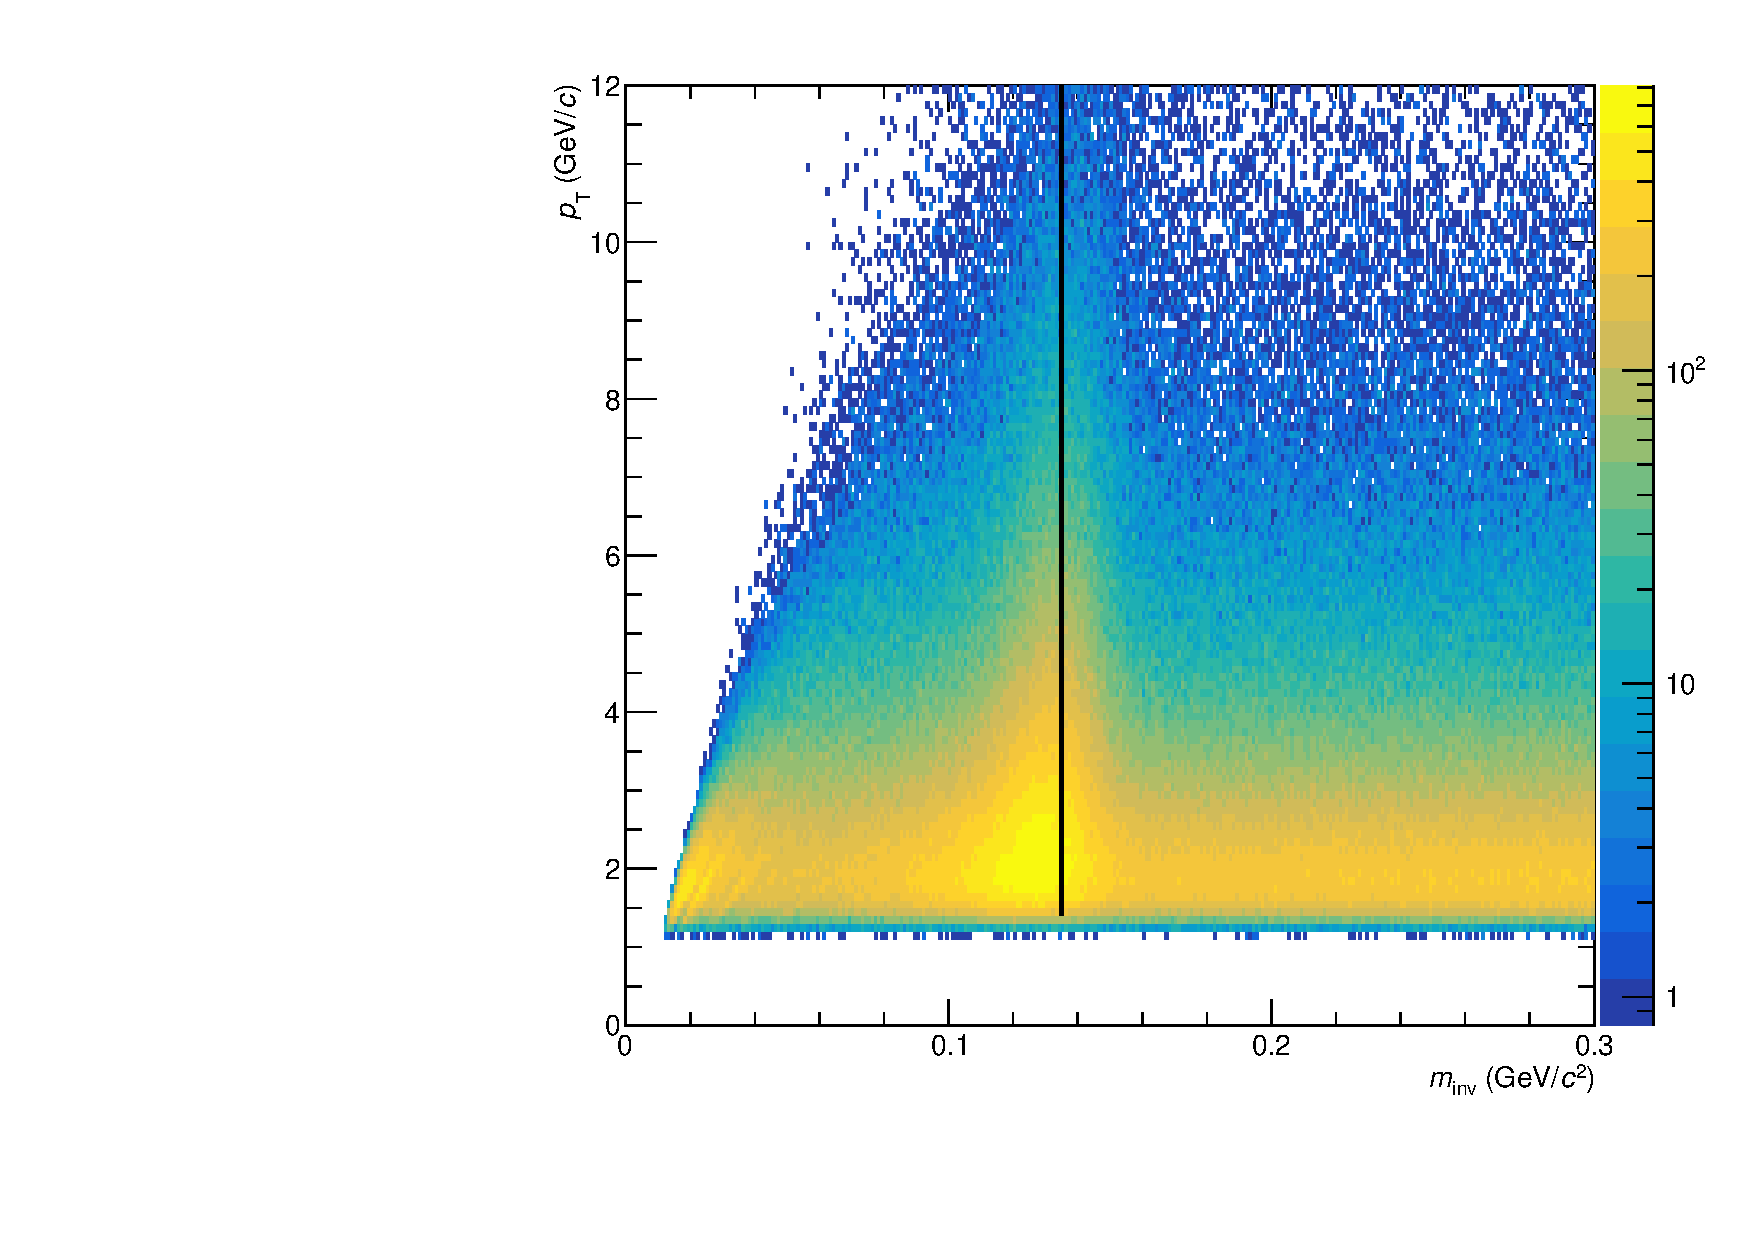
\includegraphics[width=.7\linewidth]{hInvMass_pT_Signal.pdf}
\caption{$p_\text{T}$ und $m_\text{inv}$ als Funktion der Anzahl von kombinierten  Cluster-Paaren aus der gleichen Kollision.
Die rote Linie bei $m_{\text{inv}}\approx0\,135\text{ GeV/}c^{2}$, indiziert die $\pi^{0}$ Masse, wo sich eine deutliche Häufung der Einträge abzeichnet.
Die schwarzen Linien stellen die Grenzen der $p_{\text{T}}$-Intervalle dar.}
\label{figInvMassPt_a}
\end{figure}
\newline
Um die Anzahl der $\pi^{0}$ zu messen, werden von \textit{Clusterpaaren} $m_\text{inv}$ und $p_\text{T}$ nach Gleichungen \ref{eq_invmass} und \ref{eq_pt} bestimmt.
Da die Information fehlt, ob und welche \textit{Cluster} von einem Teilchen aus dem Zerfall eines $\pi^{0}$ stammen, werden alle \textit{Cluster} eines \textit{events} paarweise miteinander kombiniert.
Diese Methode wird als \textit{same Event} Methode bezeichnet.
Abbildung \ref{figInvMassPt_a} zeigt die Anzahl der \textit{Clusterpaare} in Abhängigkeit von $m_{\text{inv}}$ und $p_{\text{T}}$.
Durch die paarweise Kombination aller \textit{Cluster} eines \textit{Events} gibt es sowohl Kombinationen von \textit{Clustern} von Teilchen die über den Zerfall eines einzelnen $\pi^{0}$ zusammenhängen, als auch von \textit{Clustern} von Teilchen, die nicht über den Zerfall eines einzelnen $\pi^{0}$ zusammenhängen.
\newline
Es zeichnet sich eine Häufung der Datenpunkte um die $\pi^{0}$ Masse ab.
Dieser Häufung liegt das Signal zugrunde.
Als Signal wird die Summe aller \textit{Clusterpaare} bezeichnet, die aus einem Zerfall eines $\pi^{0}$ kommen.
Da Photonen durch Paarbildung in ein Elektron und ein Positron konvertieren können, bestehen einige \textit{Cluster} aus nur einem der beiden Konversionsprodukte.
Diese \textit{Cluster} besitzen eine geringere Energie als das eigentliche Photon besaß.
Entsprechend liegen Einträge von Kombinationen mit diesen \textit{Clustern} bei kleinerem $m_\text{inv}$, als wenn diese \textit{Cluster} aus den Photonen, die konvertiert sind, entstanden wären.
Deshalb wird bei $m_\text{inv}<0\,135\text{ GeV}/c^{2}$ ebenfalls Signal erwartet.
\newline
Alle \textit{Clusterpaare}, die nicht zum Signal zählen, werden als Untergrund bezeichnet.
Dieser wird in zwei Teile unterteilt: den kombinatorischen oder auch unkorrelierten Untergrund und den korrelierten Untergrund.
Der korrelierten Untergrund entsteht durch paarweise Kombinationen von \textit{Clustern}, zwischen denen eine Korrelation besteht.
Das heißt, dass die Teilchen, durch die die eben genannten \textit{Cluster} entstanden sind, nicht aus dem Zerfall desselben $\pi^{0}$ stammen, aber über andere Zerfälle zusammenhängen.
Durch die paarweise Kombination von \textit{Clustern} von unkorrelierten Teilchen entsteht der unkorrelierte Untergrund.
\newline
Um die Wahrscheinlichkeit zu senken, dass zwei Teilchen zu einem \textit{Cluster} zusammengefasst werden, benötigen die \textit{Cluster} dieser Teilchen eine Zellendiagonale als Mindestabstand.
Dieser Mindestabstand entspricht einem minimalen Öffnungswinkel.
Aufgrund des minimalen Öffnungswinkel gibt es für $m_\text{inv}$ eine untere Grenze die von $p_\text{T}$ abhängt, ab dem Einträge vorhanden sein können.
\newline
Die Anzahl der $\pi^{0}$ weist eine $p_{\text{T}}$-Abhängigkeit auf.
Deshalb wird die Verteilung aus Abbildung \ref{figInvMassPt_a} in einzelnen $p_{\text{T}}$-Intervallen analysiert.
Die Intervalle werden so gewählt, dass sie möglichst klein sind, während die statistischen Unsicherheiten der Datenpunkte nicht zu groß werden.
In Abbildung \ref{figInvMassPt_a} werden die $p_{\text{T}}$-Intervalle durch die schwarzen Linien gekennzeichnet.
\begin{figure}[tbp]
\centering
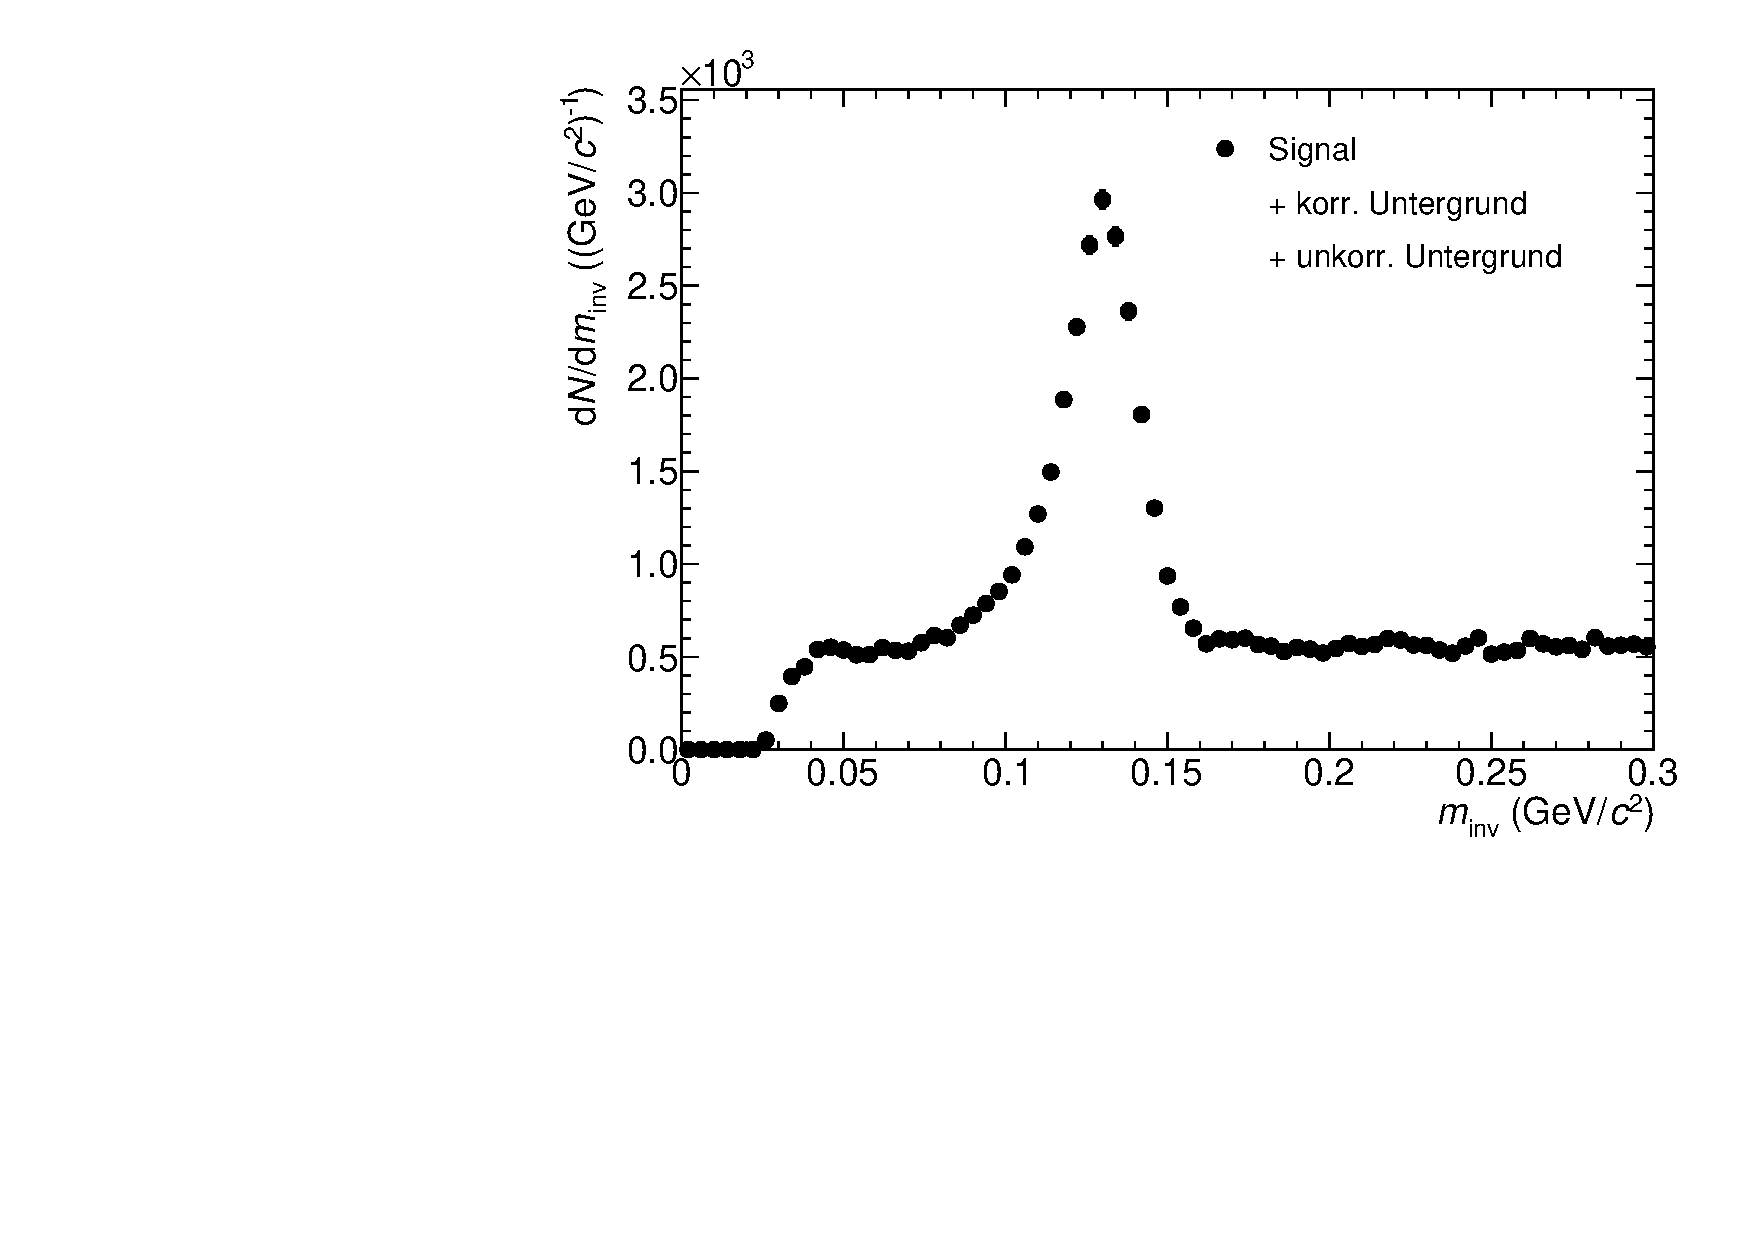
\includegraphics[width=.75\linewidth]{hSignalPlusBkg.pdf}
\caption{Projektion von Abbildung \ref{figInvMassPt_a} im $p_{\text{T}}$-Intervall $(3,2 - 3,4) (\text{GeV/}c)$. Es ist ein deutlicher Peak um $m_{\pi^{0}} \approx 0\,135\text{ GeV/}c^{2}$ zu erkennen, aber auch Untergrund, da das Signal zu höheren Massen gaußförmig abklingen sollte. Bei $m_{\text{inv}} < m_{\pi^{0}}$ kann Signal vorliegen, das aus konvertierten Photonen besteht, weshalb eine Aussage über die Form, beziehungsweise den Untergrund dort schwer möglich ist.}
\label{figSignalPlusBkg}
\end{figure}
\newline
Abbildung \ref{figSignalPlusBkg} zeigt die Anzahl der \textit{Clusterpaare} in Abhängigkeit der invarianten Masse im $p_{\text{T}}$-Intervall von $(3\,2 - 3\,4)(\text{GeV}/c)$.
Die in Abbildung \ref{figInvMassPt_a} beschriebene Anhäufung der Datenpunkten zeigt sich auch hier deutlich und wird im Folgenden als Peak bezeichnet.
Der Peak besteht wie zuvor erwähnt aus Signal.
\newline
Im folgenden Abschnitt wird eine Methode zur Abschätzung des unkorrelierten Untergrunds vorgestellt. 